%\documentstyle{llncs}
\documentclass{llncs}

\input mac.tex

\usepackage{amsmath}
\usepackage{graphicx}
\usepackage{verbatim}

\newcommand{\todo}[1]{\textbf{TODO:} $<<$ #1 $>>$}
\newcommand{\comments}[1]{}
\newcommand{\code}[1]{\texttt{#1}}
\newcommand{\af}{ActorFoundry v1.0}
\newcommand{\oaf}{Actor Foundry v0.1.14}

\title{An Efficient Actor Name Management Architecture to Support
Encapsulation, Distributed Execution and Strong Mobility}
\author{Rajesh K Karmani, Amin Shali, Gul Agha}
\institute{University of Illinois at Urbana-Champaign}

\begin{document}
\maketitle

\begin{abstract}


In order to address the problem of programming multicore
architectures, at least 15 implementations of the \emph{Actor model}
have been proposed in the past couple of years.  Most of these
implementations are in the form of libraries (written in Java, Ruby,
Python, Scala, Squeak, C++ among others) which provide runtime
support for actors.  An issue is that these runtime libraries do not
support \emph{distributed execution} and \emph{strong mobility}.
While this reduces execution overhead on shared memory multicore
computers, we argue that these actor properties are necessary for
programming \emph{scalable} multicore architectures.  Many
implementations have also compromised on \emph{enforcing} one of the
key requirements of \emph{actor encapsulation}, namely, that an actor
cannot directly access methods (or state) of another actor but may
only send messages to it.  We analyze the costs of supporting
encapsulation, distributed execution and strong mobility in
ActorFoundry, a Java library for actors, and show that the major
overhead is the result of a naive implementation of location independent
\emph{actor names}.  We then describe techniques to improve the
efficiency of distributed actor name management.  Results of our
experiments demonstrate that, using these techniques, actor properties
can be efficiently supported in libraries. We conclude by discussing
the implications of name management for garbage collection and
resource discovery.

\end{abstract}



\section{Introduction}
In the Actor model of programming \cite{ACTORS}, systems comprise of concurrent, autonomous entities called actors which do not share state.  Hence, actors are inherently free from low-level data races. Moreover, access to local state only increases the locality of reference.

The synchronization primitive in the Actor model is asynchronous message-passing.  While waiting for a lock, threads occupy system resources such as a native stack and possibly other locks. In contrast, actors waiting for a message
do not hold any system resources. Hence asynchronous message-passing is less error-prone than locks.
Moreover, the Actor model is an inherently concurrent model of programming.  Hence it is widely considered to be a promising approach towards programming scalable multi-core architectures.

Some languages based on the Actor model that are currently being used
include Erlang \cite{erlang-book}, SALSA
\cite{varela2001pdr}, Ptolemy \cite{ptolemy-actors}, E language \cite{elang}.
Additionally there are various Actor libraries written on top of existing languages like Python (Parley \cite{parley},
Stackless python), Ruby (RevActor, Dramatis, Stage \cite{stage}), C++ (Theron), Java (Kilim \cite{srinivasan2008kit},
ActorFoundry \cite{OAF}, Actor Architecture \cite{AA_Man}, JavAct \cite{Zwicky}, Jetlang, Jsasb, Actors Guild), Scala \cite{haller2007aut}, and .NET (Microsoft's Asynchronous Agents, Retlang).

While the above-mentioned languages and libraries support concurrent entities and asynchronous message-passing, many of them overlook some key semantic properties of the Actor model of programming. These properties include encapsulation, distributed execution and strong mobility. Encapsulation is important for reasoning about safety properties. It also enables modular analyis and higher software maintainability. Modular reasoning allows composition of software components which in turn enables building large-scale open systems. Distributed execution and strong mobility facilitates load-balancing and fault-tolerance. Also, support for distribution allows a uniform programming model for multicores as well as the Internet. We would present arguments that support for distributed execution is important for programming scalable multicore architectures.

There is a debate going on whether the right model to program multicore architectures is a shared memory model or through message-passing. Due to the desirable properties of data race freedom and aynschrony, we believe that the right model is Actor model and hence, we belong to the message-passing camp. More than that, we believe that even the design and implementation of tools and run-time for multicores should also assume a distributed memory model. As the number of cores on a chip grow and we move towards \emph{manycore} architectures, the logic and circuitry required for cache-coherence does not scale. For the software, assumption of a shared data structure by the parallel tasks can create bottlenecks (due to locks and other forms of synchronization) which may prevent exploiting the parallelism of an application. Conceptually, even the hardware cache is a shared data structure, only that it is managed by the hardware \cite{mit-fos}. 

Such observations and other related problems have prompted the design of services based run-time and operating systems \cite{mit-fos,singularity,servo}, where the services communicated by message-passing. We would term these services as coarse-grained actors. Therefore, we believe that support for distributed execution is important for achieving scalable performance on manycore, heterogeneous architectures, specially for dynamic, irregular apps \cite{jpdc94}. We believe that distributed execution and mobility enable a separation of concerns: ``what'' from ``where''.

%All the examples here with details about semantics

A survey of existing JVM-based Actor frameworks including Scala and Kilim shows the lack of these properties though. We describe a na\"ive implementation of encapsulation, distributed execution and strong mobility in the context of ActorFoundry, an Actor library for Java. We present a detailed analysis of the various costs. We identify the key sources of inefficiency in implementing these properties: mapping of actors to Java threads and location-independent naming. The first problem is addressed effectively in Kilim \cite{srinivasan2008kit} through a Continuations Passing Style (CPS) transform on Java bytecode. The transform exploits properties of actors such as lack of shared state and message-driven scheduling, and hence allows light-weight actors that can be efficiently migrated.

In this paper, we focus on supporting location-independent naming in Actor systems. We discuss why efficiently providing location-independent naming can be a challenge. The major considerations are space requirement and how naming affects garbage collection in Actor systems. The map of Actor name to its state (including its execution stack and the mailbox) can grow unbounded in the absence of an Actor garbage collector. As previous literature suggests \cite{iwmm92}, Actor garbage collection in distributed settings is an expensive task. Hence this presents an additional barrier towards providing support for distribution and strong mobility in Actor systems. Maps with weak references \cite{weakrefs} allow such mapping with the facility that if the Actor name is not reachable outside the map, the JVM garbage collector can remove the entry from the map. Hence, JVM GC effectively doubles as the local Actor GC. But in the presence of distribution and mobility, the names can be shared with remote JVMs and \code{equals()} method for Actor name object does not check for reference equality. Hence weak maps can not be employed. %Moreover, a global lookup table is a potential source of bottleneck for different threads running on a shared-memory multicore node.

In order to mitigate these inefficiencies, we refer to the concepts of 'receptionists' and 'external actors' as described in \cite{agha1997fac}. We argue that only the receptionists actors need to be added to the tables. Hence the task of maintaining the tables faithfully follows the semantics of Actor operations that update the set of receptionists. We observe that while the semantics for message sends correctly update the set of receptionists and external actors, the semantics for creating and initializing new actors do not consider remote hosts. We provide the correct semantics for actor creation and initialization, as well as semantics for migration in distributed Actor systems.

\begin{comment}

\begin{align*}
%Inspiration from Actor configurations
&< \mbox{remote\_create : a, a'} > \\
&\quad \cnfg{\alpha, [R[\mbox{create(node)}]]_{a}}{\mu}{\rho}{\chi} \mapsto \cnfg{\alpha, [R[nil]]_{a}}{\mu}{\rho}{\chi \cup \{a'\}}\\
\\
&< \mbox{remote\_init : a, a'} > \\
&\quad \cnfg{\alpha, [R[\mbox{initbeh(a', v)}]]_{a}}{\mu}{\rho}{\chi} \mapsto \cnfg{\alpha, [R[nil]]_{a}}{\mu}{\rho \cup (FV(v) \cap Dom (\alpha))}{\chi}\\
\\
&< \mbox{remote\_create\_request : a, a'} > \\
&\quad \cnfg{\alpha}{\mu}{\rho}{\chi} \mapsto \cnfg{\alpha, (?_a)_{a'}}{\mu}{\rho \cup \{a'\}}{\chi}\\
\\
&< \mbox{remote\_init\_request : a, a'} > \\
&\quad \cnfg{\alpha, (?_a)_{a'}}{\mu}{\rho}{\chi} \mapsto \cnfg{\alpha, (v)_{a'}}{\mu}{\rho}{\chi \cup (FV(v) - Dom (\alpha))}\\
\\
&< \mbox{migrate\_out : a, node} > \\
&\quad \cnfg{\alpha, [R[\mbox{migrate(node)}]]_{a}}{\mu}{\rho}{\chi} \mapsto \cnfg{\alpha}{\mu}{(\rho \cup (FV(a) \cap Dom (\alpha))) - \{a\}}{\chi}\\
\\
&< \mbox{migrate\_in : a} > \\
&\quad \cnfg{\alpha}{\mu}{\rho}{\chi} \mapsto \cnfg{\alpha, [R[nil]]_{a}}{\mu}{\rho \cup \{a\}}{\chi \cup (FV(a) - Dom (\alpha))}
\end{align*}
\end{comment}

Using these semantics, we describe and implement techniques that dramatically reduce the space-related inefficiencies. We briefly describe a proof of its correctness. We also describe how the JVM GC doubles as a local Actor garbage collector without weak maps using our approach. We also argue that generic clustering frameworks like Terracotta can not be more efficient since they do not exploit Actor semantics of encapsulation and locality. Evaluation of costs in the context of a JVM-based Actor library suggests that overhead of these semantics is negligible even in the case of a library implementation. 


% Separate concerns: advantages of distributed execution, mobility, load-balancing scheduler,
In the next three sections, we discuss the significance of each of encapsulation, distributed execution and strong mobility in Actor systems and what each of them requires from an Actor naming architecture. Next, we present the results from evaluation of a na\"ive implementation of these requirements. We identify the key reasons of inefficiency and propose optimizations that satisfy the requirements imposed by the properties. Next, we presents our results from evaluating our approach for a number of parallel and concurrent benchmarks. In the end, we conclude with related work in other Actor implementations and discuss future directions for research.
 

\section{Encapsulation}
Encapsulation is one of the core principles of object-oriented programming. Preserving encapsulation boundaries between objects facilitates reasoning about safety properties like memory safety, data race freedom, safe modification of object implementation.
%Safety is an overloaded term and has been used in the context of both language and program. 
For example, Java is termed as a memory-safe language because it hides memory pointers behind object references which provide safe access to objects. This turns out to be important in order to preserve object semantics which require access to object state using well-defined interfaces. %Another perceived dimension to Java's safety is type-safety. We do not intend to discuss Java's safety features here but we try to convey the point that safety is a broad term. 

%In the context of programs, safety properties describe invariants that should hold in each state of program execution. These are usually properties about semantics of the program rather than a programming model or language.


In the context of the Actor model of programming, we group two core properties of the model under Actor encapsulation. The first one being that there is no shared state among actors. Secondly, an actor can access the state of another actor only by message-passing.

It is very tempting to ignore these semantics in the quest of an efficient implementation of Actor semantics. The temptation is stronger in the case of a library implementation compared to a language implementation. For example, in order to ensure that an actor is unable to access the state of another actor directly, a language may use an abstraction like mailbox address or a channel but use direct references in the compiled code for efficiency. This is similar to how Java uses object references to abstract away pointers. In an actor library, such abstractions (or indirection) have to be resolved at run-time which is more expensive. 

For example, the following code demonstrates violation of one of the core Actor property due to lack of enforcement of Actor encapsulation in the Scala actors library. The main actor, in addition to sending an \code{enter()} message, executes \code{enter()} in its own stack. On a multi-threaded, shared memory implementation of the Actor model, this violates the actor semantics that an actor can only update its local state by processing one message at a time. This can lead to an inconsistent state and manifest into an error.

\makebox[\textwidth]{\hrulefill}
\begin{footnotesize}
\begin{verbatim}
import scala.actors.Actor
import scala.actors.Actor._

object sempahore {
    class SemaphoreActor() extends Actor {
        var MAX = 1;
        var num = 0;

        def act() { 
         loop { react {
                case ("enter") => {
               enter()
                }
                case ("other") => {
                    System.exit(0);
                }
        }}}

        def enter() {
          if (num  < MAX) {
            // critical section
            num = num + 1;
          }
        }
    }

    def main(args : Array[String]) : Unit = {
       var gate = new GateActor()
       gate.start
       gate ! "enter"
       gate.enter
    }
}
\end{verbatim}
\end{footnotesize}
\makebox[\textwidth]{\hrulefill}


We believe that the two aspects of Actor encapsulation are important for writing large-scale Actor programs. It is difficult to provide semantics for and reason about Actor languages not guaranteeing these encapsulation boundaries. \todo {Private conversation with Mirko regarding providing semantics for Scala, which does not guarantee these two aspects.}

In this paper, we focus on how to enforce the property \emph{in a library implementation} that an actor cannot directly access methods (or state) of another actor but may only send messages to it. The problem in this respect is that libraries written on top of existing object-oriented languages represent actors as objects, and the host language can not prevent an actor object from directly calling visible methods on another actor object. We believe that the correct approach is to employ indirect addressing through Actor name objects. A new creation and initialization procedure may be required that returns reference to an Actor name object instead of that to an Actor object. When an actor sends a message to the Actor name, the run-time resolves the name to a mailbox and delivers the message.

\begin{figure}%[htb]
\centerline
{
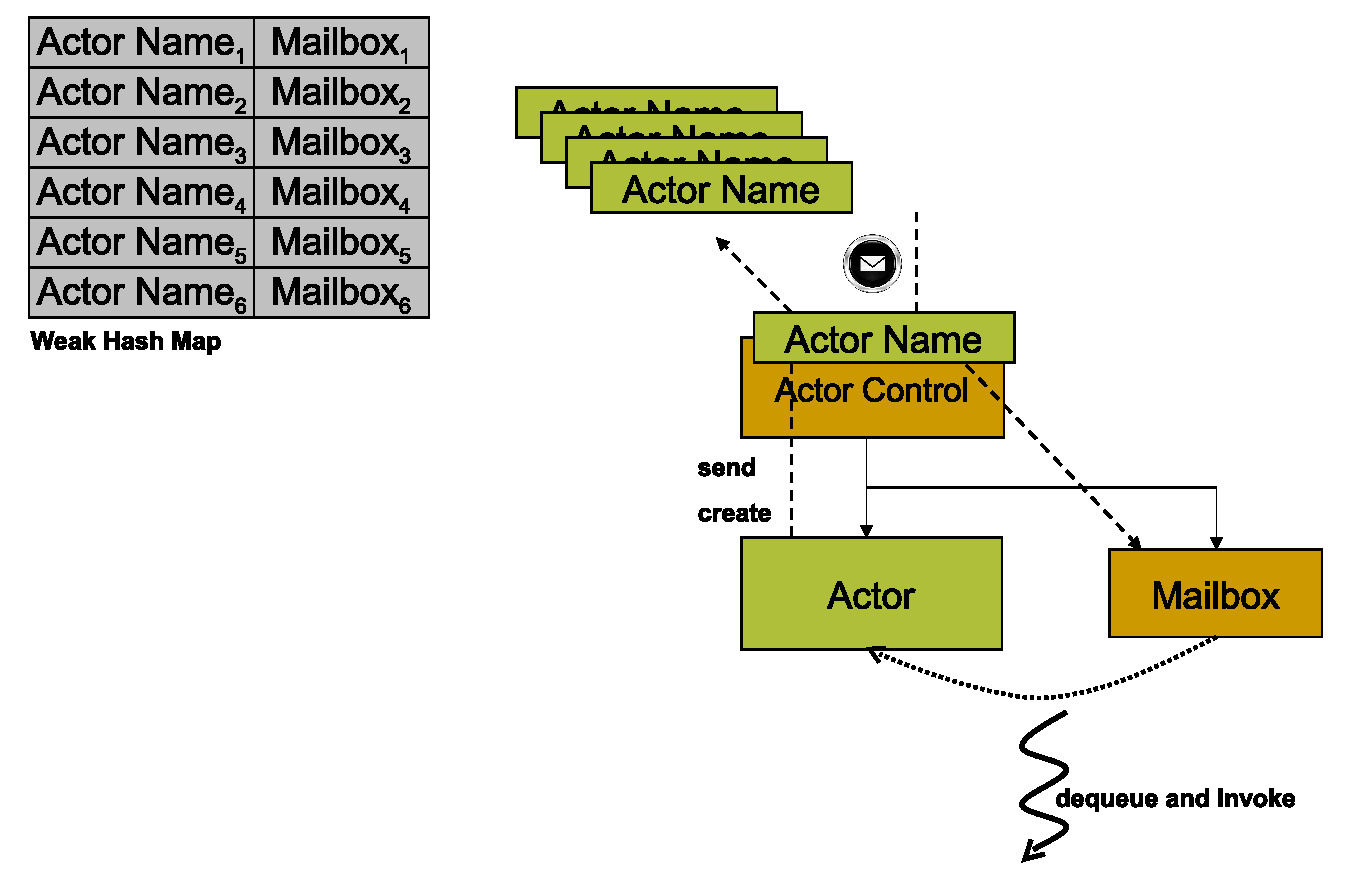
\includegraphics[scale=0.4]{images/escape1.eps}
}
\caption{Actor node using name table with weak references to support encapsulation.}
\label{local_node}
\end{figure}


A simple mechanism is to store the pair of Actor name and mailbox in a hash table. A problem with this approach is that the table can grow unbounded in the absence of an Actor garbage collection mechanism. For example, in Java's implementation of hash tables, each entry in the table would occupy 16 bytes, More importantly though, in the absence of an Actor garbage collection mechanism, an entry in the table means that the actor's state, mailbox and continuation will remain in the memory forever, even if no actor knows its name anymore.


Assuming no support for distributed execution, a more effective solution on platforms with object garbage collection facility, is to use tables with weak references \cite{weakrefs}. Maps with weak references facilitate the following desirable characteristic: the object GC is allowed to remove the Actor name and the corresponding mailbox from the table if the Actor name is not reachable except through the weak reference from inside the table. Hence, the object GC effectively doubles as an Actor GC on a single shared-memory node. An Actor system constituting name tables with weak references is shown in Fig \ref{local_node}

%There is one caveat specific to library implementations; interoperability with existing code can violate encapsulation. For example, a JVM framework which is used by a group of actors and internally employs a stateful singleton object, in effect introduces shared state among actors.

\section{Distributed Execution}
Actor model is based on asynchronous message-passing between independent actors. Hence it provides a uniform model of computation for parallel as well as distributed computing. Apart from programming naturally distributed applications like P2P, sensor networks and Internet computing, distribution is important for parallel performance on scalable multicore architectures. Support for distributed execution is also imperative for mobility.

Distributed execution requires strong references inside the name tables. The reason being that Actors may not be known by any actor inside their node but actors at other hosts may have references to it. Hence, a garbage collector running on the local host may incorrectly remove an entry of an actor from the name table with weak references, and render future messages to the actor from remote actors undeliverable. An Actor system with name tables is shown in Fig \ref{dist_node}.


\begin{figure}%[htb]
\centerline
{
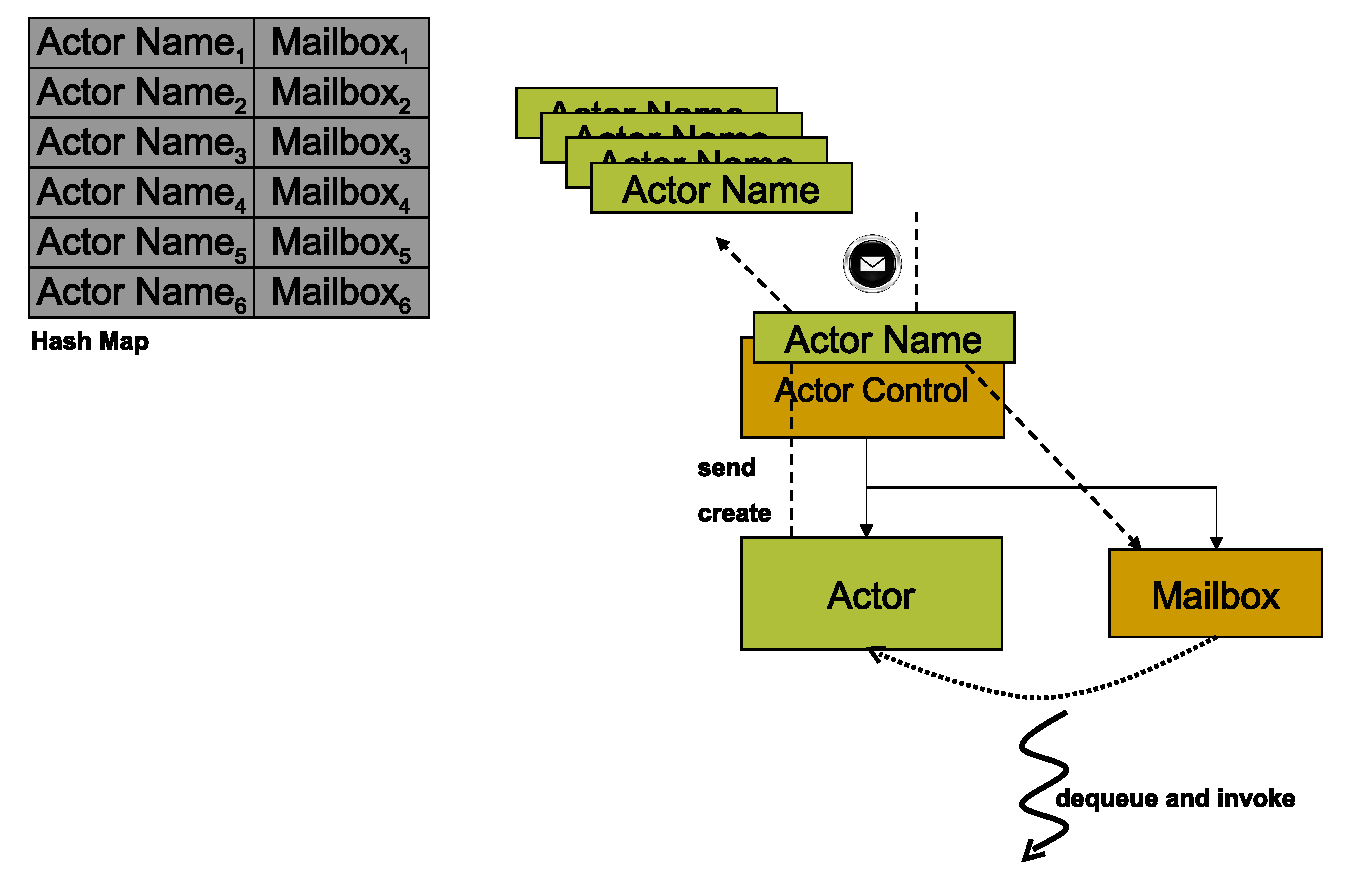
\includegraphics[scale=0.4]{images/escape2.eps}
}
\caption{Actor node with name table to support distributed execution.}
\label{dist_node}
\end{figure}


%\code example - Weather widget talking to weather server

%\subsection{Location Transparency}

\section{Strong Mobility}

Proponents of Actor model emphasize transparent distribution of Actor programs, making the programs elegant and the task of the programmer less arduous. Actor systems should be able to provide facilities like load-balancing and fault-tolerance while keeping a uniform location-independent naming model for programmers. This in turn separates the concern of ``what'' from ``where'' and enables optimizations by the system based on run-time conditions.

Mobility is defined as the ability of computation to move across different nodes. In their seminal work, Fuggetta et al. classify mobility as either strong or weak \cite{mobility}. Strong mobility is defined as the ability of a system to support movement of both code and execution state. Weak mobility, on the other hand, allows movement of only code. Initial state may be transferrable though in weak mobility.

At the system level weak mobility is essential for achieving load-balancing, facilitating fault-tolerance, reconfiguration. Previous work has shown that location transparency and mobility can be essential for achieving scalable performance, specially for dynamic, irregular applications over sparse data structures \cite{jpdc94}. In such applications different stages may require a different distribution of computation. In other cases, the optimal distribution is dependent on run-time conditions such as data and work load. The ability to dynamically redistribute computation requires support for mobility.

We also believe that strong mobility enables declarative exploitation of heterogeneous system resources such as GPUs, DSPs, other task-specific accelerators, high clock frequency cores, (when augmented with discovery services). It leads to elegant programming and simpler control flow.

\makebox[\textwidth]{\hrulefill}
\begin{footnotesize}
\begin{verbatim}

actor MatrixMultiply {
  message start(int N) {
   // Random generation of A, B
   
   migrate("gpu");

   int [][] C = new int [N][N];
   create <N * N> MultiplyActor()<-start(A, B, C);

   migrate("cpu");
   // print C

  }
}

actor MultiplyActor {
  int id;
  message multiply (int [][] A, int [][] B, int [][] C) {
    int i = id % N, j = id / N;
    C[i][j] = A[i][j] * B[i][j];
  }
}

\end{verbatim}
\end{footnotesize}
\makebox[\textwidth]{\hrulefill}


It can also express streaming-code algorithms where the programmer wishes to move code rather than data. In combination with data discovery services, mobile actors can process data in-place. This may be preferable due to privacy reasons or that it is more efficient to move code rather than data. This is quite similar to pipeline processing except that the conceptual model is reversed: transformation actors processing the statically residing data one after the other. Moreover, this model by definition has ownership transfer semantics for messages, which as discussed earlier can be implemented more efficiently.
%Having strong mobility as a primitive helps the programmer e

Mobility is quite natural to the Actor model due to modularity of control and encapsulation. Object-oriented languages may allow mobility at the level of objects but all thread stacks executing methods on the object need to be made aware of this migration. Moreover, when the stack frame require access to the object on a remote node, the execution stack is moved to the remote node, complete the execution of the frame and then migrated back to the original node \cite{walsh2000spm}.


A protocol for supporting mobility in Actor systems has been described in \cite{sc95}. It requires Actor names to be mapped to be mapped to their possible host. Hence, in addition to name table for looking up the Actor state, an Actor system requires another name service that can lookup the host (physical address) of an Actor. An Actor system with name tables is shown in Fig \ref{mobile_node}.

\begin{figure}%[htb]
\centerline
{
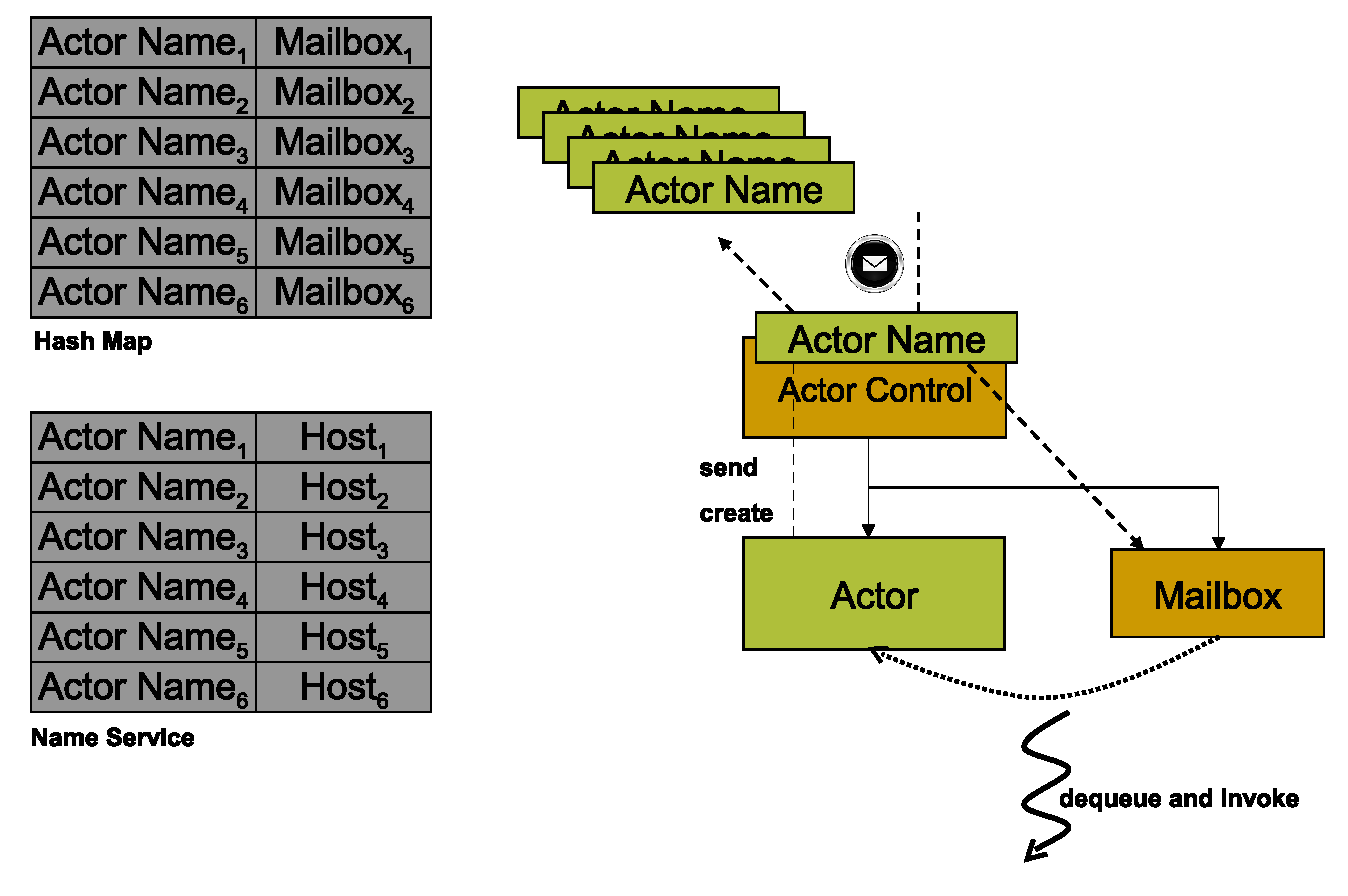
\includegraphics[scale=0.4]{images/escape3.eps}
}
\caption{Actor node with name table and a name service to support mobility}
\label{mobile_node}
\end{figure}


\section{Implementation}
\label{sec-implementation}
We will discuss Actors semantics in the context of a JVM-based Actor library called \af{}. \oaf{} was originally designed and developed at the Open Systems Laboratory by Mark Astley along with Thomas Clausen and James Waldby around 1998-2000 \cite{OAF}. The goal was to develop a modular Actor library for a new, upcoming object-oriented language called Java. \oaf{} has a simple, elegant model in which the control and mailbox are hidden away in the library while the programmer is concerned with an Actor's local state and behavior only \ref{actor_anatomy}. To leverage the actor semantics, the programmer is provided with a small set of library methods as part of the \oaf{} API. This includes:
\begin{description}
 \item[\code{send(actorAddress, message, args)}]
Sends an asynchronous message to the actor at specified address along with arguments. The argument message is a String which should match a method name in the target actor behavior, otherwise an exception is thrown at run-time.
 \item[\code{call(actorAddress, message, args)}]
Sends an asynchronous message and waits for a reply. The reply is also an asynchronous message which either contains the return value or simply an acknowledgement. 
 \item[\code{create(node, behavior, args)}]
Creates a new actor with the given behavior at the specified node. The argument node is optional. In case it is not specified, the actor is created locally. The arguments are passed to the constructor.
\item[\code{destroy(note)}]
An explicit termination of the current actor. This is provided as an alternative to an automatic actor garbage collection mechanism.
\item[\code{self()}]
Returns the address of the current actor.
\item[\code{migrate(node)}]
Requests the run-time to schedule the current actor for migration to a remote node. \oaf{} only supports weak mobility, hence the actor is migrated at message processing boundaries only.
\item[\code{cancelMigrate()}]
Cancels an earlier request for migration.
 \end{description}


Behind the scenes, \oaf{} maps each actor onto a JVM thread (1:1
architecture). Messages are dispatched to actors by using the Java
Reflection API. This can technically be termed as pattern-matching
since the message string is matched to a method name at run-time and
the method is selected based on the run-time type of arguments
\cite{multijava}. Though, it is certainly not as expressive as the
pattern-matching in Erlang \cite{erlang-book} and Scala
\cite{haller2007aut}. Any Java object can be part of a message in
\oaf{}; the only restriction being that the object implements
\code{java.lang.Serializable} interface. All message contents are sent
by making a deep copy by using Java's Serialization and
Deserialization mechanism.

\oaf{} also supports distributed execution of actor programs, location independence and weak mobility \cite{mobility}. In addition, \oaf{} logs system and library events to the local file system. 

%While this implementation faithfully preserves actor semantics like fairness (as fair as the underlying JVM and OS scheduler), encapsulation, location independence and mobility, it makes the execution overhead of actor programs prohibitively high, making \oaf{} infeasible to use. In order to gauge the performance of \oaf{}, we implement a small benchmark called Threadring \cite{lang-shootout} in which 503 concurrent entities pass a token around in a ring 10 million times. Threadring provides a crude estimate of actor creation overhead and stress tests the message-passing and context switch. When we ran this benchmark, it took about 780s \todo{verify on Amin's machine} to finish. In contrast, an Erlang implementation takes about 10s while a Java Thread implementation takes 150s \todo{verify on Amin's machine}.

This implementation faithfully preserves Actor semantics like fairness (as fair as the underlying JVM and OS scheduler), encapsulation, location independence and mobility. In order to gauge the performance of \oaf{}, we implement a small benchmark called Threadring \cite{lang-shootout} in which 503 concurrent entities pass a token around in a ring 10 million times. Threadring provides a crude estimate of actor creation overhead and stress tests the message-passing and context switch. 

For our experiments we use a Dell XPS laptop with Intel Core\texttrademark{} 2 Duo CPU @2.40GHz, 4GB RAM and 3MB L2 cache. The software platform is Sun's Java\texttrademark{} SE Runtime Environment 1.6.0 and Java HotSpot\texttrademark{} Server VM 10.0 running on Linux 2.6.26. We set the JVM heap size to 256MB for all experiments unless specified. Upon running this benchmark, we find it takes about 695s to finish. In contrast, an Erlang implementation takes about 8s while a Java Thread implementation takes 63s. See Figure \ref{tr_performance_orig_af} for a full comparison.
\begin{figure}%[htb]
%\begin{center}
\centerline
{
%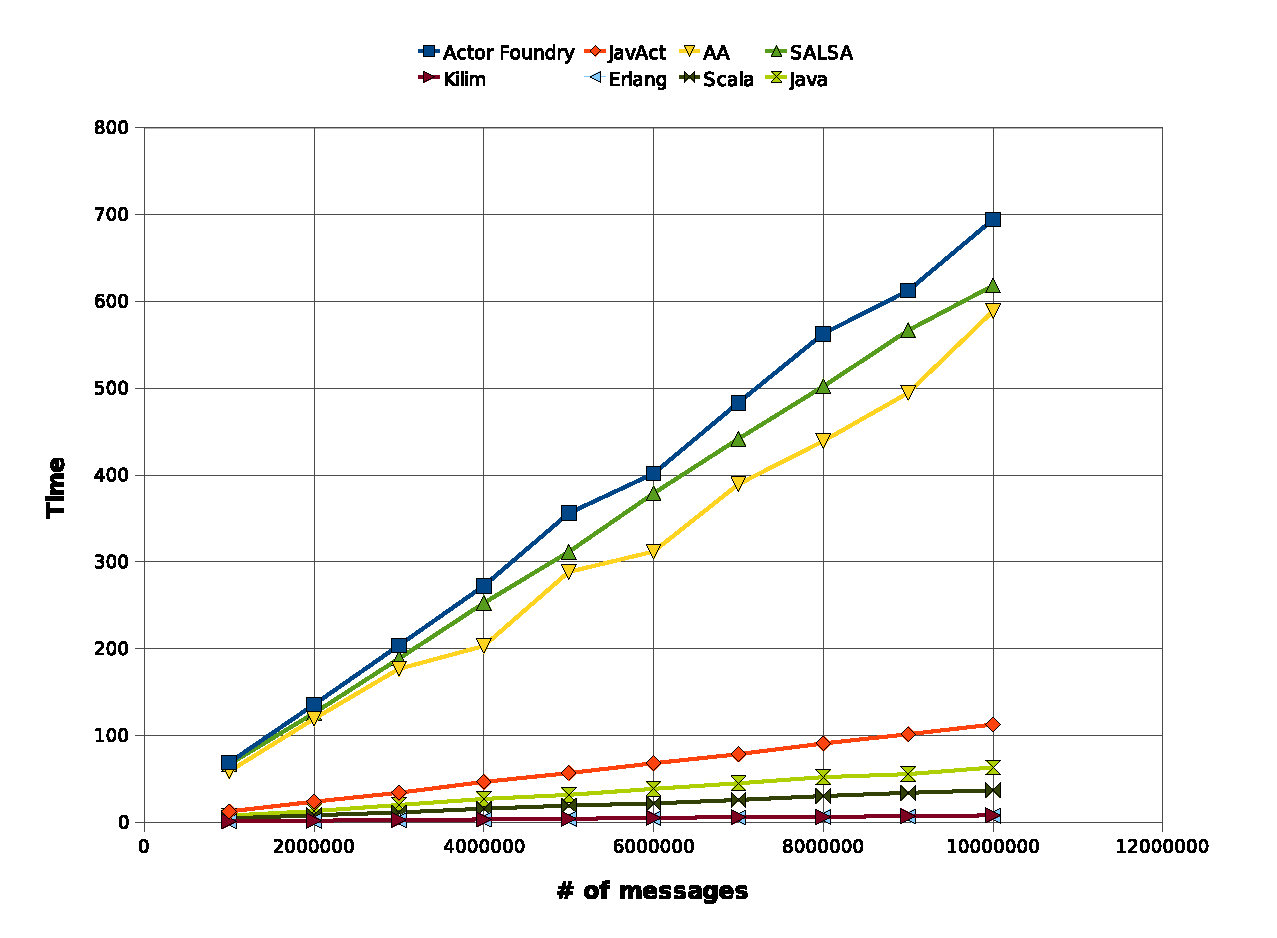
\includegraphics[bb=0 0 597 434, scale=0.55]{images/tr_performance_old_af.eps}
% tr_performance_old_af.eps: 0x0 pixel, 300dpi, 0.00x0.00 cm, bb=0 0 597 434
}
%\end{center}
\caption{Threadring Performance - \oaf{} compared with other concurrent languages and libraries}
\label{tr_performance_orig_af}
\end{figure}
This shows that a faithful but na\"ive implementation of Actor semantics can make the execution overhead of Actor programs extremely high, making \oaf{} feasible only for coarse-grained conccurent or distributed applications. We observe a similar execution overhead for SALSA and Actor Architecture. On the other hand, Kilim and Scala actors library perform an order of magnitude faster. JavaAct performs much better than \oaf{} but does not come close to either Kilim or Scala in terms of efficiency.

\subsection{Continuations based Actors}

Prior experience with ThAL language \cite{wkim-phd} suggests that continuations based actors would provide significant improvement in terms of creation as well as context switch overhead. We integrate Kilim's light-weight Task class and its bytecode post-processor (``weaver'') into \af{}. This transformation presents two challenges.

To begin with, the transform would not work when messages were dispatched using Java Reflection API. The reason being that the weaver is unable to transform Java library code and this prevented the continuations to be available in the actor code. To overcome this, we generate custom reflection for each actor behavior. It finds the matching method by comparing the message string to method's name and the type of message arguments to method's formal arguments' type. Once a match is found, the method is dispatched statically. As a pleasant side-effect, it is more efficient than Java Reflection. 

Secondly, the transform also require introducing a scheduler for \af{} which is aware of cooperative, continuations-based actors. The scheduler employs a fixed number of JVM threads called worker threads. All worker threads currently share a common scheduler queue. Each worker thread dequeues an actor from the queue and call its continuation. Actors are assumed to be cooperative; an actor continues to run until it yields waiting for a message. In order to increase locality and reduce actor context switches, an actor can process multiple messages while being scheduled. On the other hand, this can cause starvation in the system. Scheduling is message-driven only. An actor is put on the scheduler queue if and only if it has a pending message. 

With this implementation, the running time for Threadring comes down to about 267s.

\subsection{Message-passing semantics}
\label{messaging}

We profile the execution to identify further performance bottlenecks. Profiling makes it apparent that the deep copying of message contents is by far the biggest bottleneck. The faithful implementation of message-passing semantics means that message contents are deep-copied using Java's Serialization and Deserialization mechanism, even for immutable types. We disable deep-copying for some known immutable types. These included \code{java.lang.Integer}, \code{java.lang.String} and others. This further brings down the running time of Threadring to 30s. The reason behind this significant improvement is that actors in Threadring pass a token which is basically an integer representing the remaining number of passes.


We add two new methods to \af{} library: \code{sendByRef()} and \code{callByRef()} to overcome this inefficiency. These methods allow the programmer to explicitly declare transfer of ownership semantics for messages. This enables the run-time to implement such message efficiently on shared-memory systems by passing a reference.

\subsection{Na\"ive Implementation}
\subsubsection{Distribution and Location-Independent Addressing}
In \oaf{}, distributed execution is supported by means of a Transport layer. With its extensible architecture, either UDP or TCP based transport layer can be used. A node manager can communicate with another node manager by requesting its actor address through a lookup service called Yellow Page Service. The pre-requisite is that the service is running at the target node at the specified port. 

The client node can cache the manager's address locally. This address can now be used to send requests for creating actors remotely and migrating actors to the target node. This is where the power of location-independent addressing comes into play. Remote actor creation is a blocking operation that returns a location-transparent actor address. An actor on the client node can send send further messages to this actor on the remote node. It can also share this address with other actors and in turn they can send messages to this address without ever worrying about its physical location. 

In case a local actor migrates to a remote node, other actors that know this actor's address can continue to send messages to this actor. This location-independent addressing is enabled by using a protocol based on name tables, similar to the one discussed in \cite{sc95}.

\subsubsection{Mobility}
% Singularity: internal aliasing -> a complicated static analysis to ensure owernship transfer semantics

% TAlk about language based (Erlang run-time) implementation of these semantics. Static and Dynamic properties of Erlang process
\subsection{Optimizations}




%\section{Cost Evaluation}
\section{Performance}
Figure \ref{tr_performance} compares the performance of optimized implementation of ActorFoundry with Scala, Kilim, SALSA and Actor Architecture. Figure \ref{cham_performance} provides a similar comparison for Chameneos-redux benchmark. \todo{Need to compare the size/memory footprint of the run-time, each actor and each message to understand cache-related effects.}

\begin{figure}%[htb]
%\begin{center}
\centerline
{
%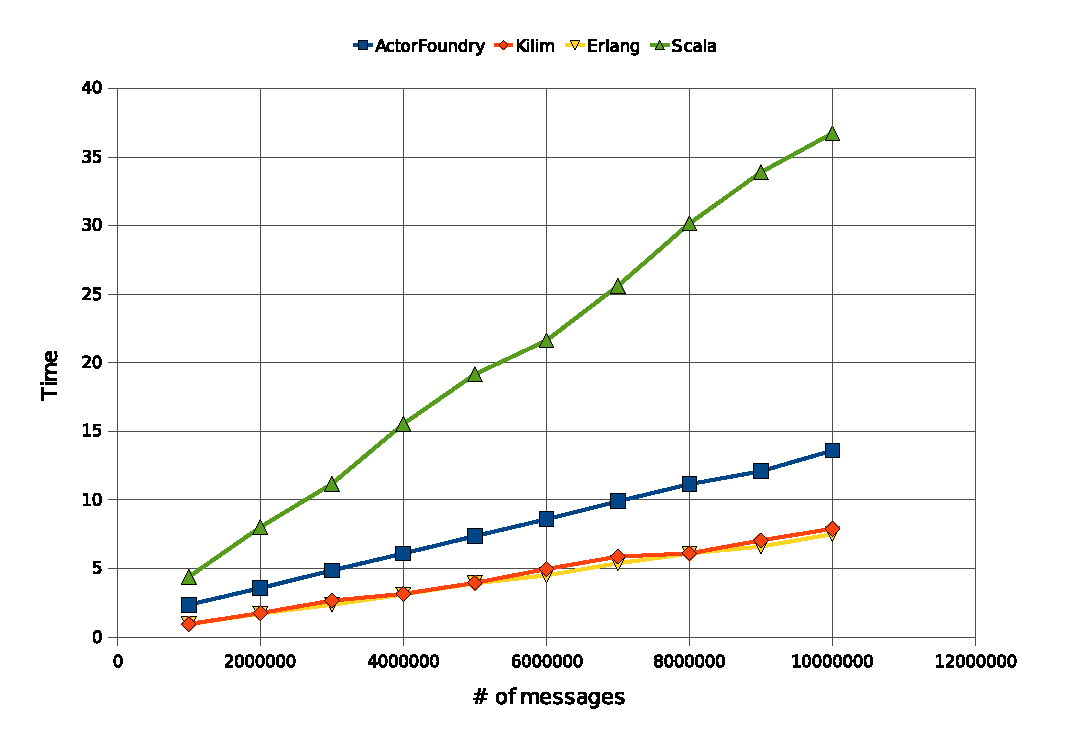
\includegraphics[bb=0 0 500 339,scale=0.70]{images/tr_performance.eps}
% tr_performance.eps: 0x0 pixel, 300dpi, 0.00x0.00 cm, bb=0 0 500 339
}
%\end{center}
\caption{Threadring Performance}
\label{tr_performance}
\end{figure}
\begin{figure}%[htb]
%\begin{center}
\centerline
{
%\includegraphics[bb=0 0 500 339,scale=0.70]{images/broker_performance.eps}
% broker_performance.eps: 0x0 pixel, 300dpi, 0.00x0.00 cm, bb=0 0 500 339
}
%\end{center}
\caption{Chameneos-redux Performance}
\label{cham_performance}
\end{figure}

We implement distributed versions of Threadring, Chameneos-redux, Na\"ive fibonacci and Red-Black ordering. We present the results of running these on a cluster of 1 to 4 nodes.

\section{Related Work}

\section{Discussion and Future work}

Discuss Erlang, ThaL and Terracotta here.

Erlang does not support strong mobility but has fault-tolerance aspect (node restart).



\bibliographystyle{unsrt}
\bibliography{actors}

\end{document}



